\chapter{Nodos de recepción} \par 

\section{Descripción general}

En este capítulo haremos un análisis profundo sobre el funcionamiento de los nodos en el sistema de detección de inhibidores
de alarma de autos. Para comenzar con el mismo es importante preguntarse: ¿qué funciones debe cumplir un nodo en el sistema?
La respuesta a esto es evidente, en el nodo se producirá la recepción de la señal de RF mediante el módulo CC1101 de Texas 
Instruments, luego de esto la demodulación ASK efectuada por el receptor será procesada en el microcontrolador seleccionado
para determinar si hay o no inhibición según estrategias más adelante detalladas y este se encargará de realizar la 
comunicación mediante el protocolo RS485 con la central de procesamientos. Integrado en el nodo se utilizan tres protocolos 
de comunicación: en primer lugar tenemos la comunicación SPI que se encarga de la interacción entre el microcontrolador y 
el receptor seleccionado; esta comunicación se utiliza para configurar los registros del CC1101 para establecer el modo de
trabajo deseado. En segunda instancia tenemos comunicación serial asíncrona entre un pin de salida del receptor por el cual 
se mandan los datos RAW de demodulación en el canal seleccionado y en último lugar tenemos el protocolo RS485 para la comunicación
de la red armada. 

\section{Prototipo}

El proceso de obtener un sistema sólido y que responda a las necesidades planteadas llevó consigo la necesidad de elaborar
dos modelos distintos de nodo. En un comienzo se buscó que el mismo tenga una realimentación visual de las mediciones tomadas,
por lo que, además de procesar las señales mediante las estrategias de detección establecidas, se asignaron salidas en seis leds
que se encargaban de indicar la potencia de RF medida con el RSSI como se puede observar en la figura \ref{prototipo_nodo}. \par 

\begin{figure}
	\centering
	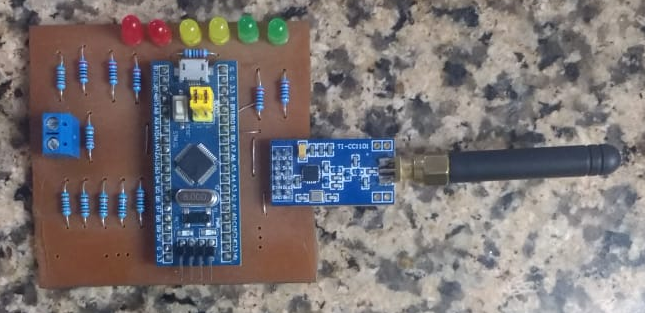
\includegraphics[scale=0.53]{images/nodos/prototipo_nodo.png}
    \caption{Primer placa del nodo armada}
	\label{prototipo_nodo}
\end{figure}

Como se puede observar el prototipo es bastante rudimentario, las placas fueron fabricadas de manera casera y sin tener grandes
cuidados en los detalles. De igual modo este diseño bastó para pulir las imperfecciones que poseía en camino al desarrollo final.\par 
Para el diseño del esquemático nos hemos basado en las prestaciones que nos brinda el microcontrolador STM32F106C8T6. El mismo
cuenta con comunicación SPI y serial integradas, por lo que haciendo uso del entorno de programación propio del fabricante 
(STM32 Cube IDE) hemos asignado los pines respectivos a cada comunicación, como se puede observar en la figura \ref{asignacion_pines}. \par

\begin{figure}
	\centering
	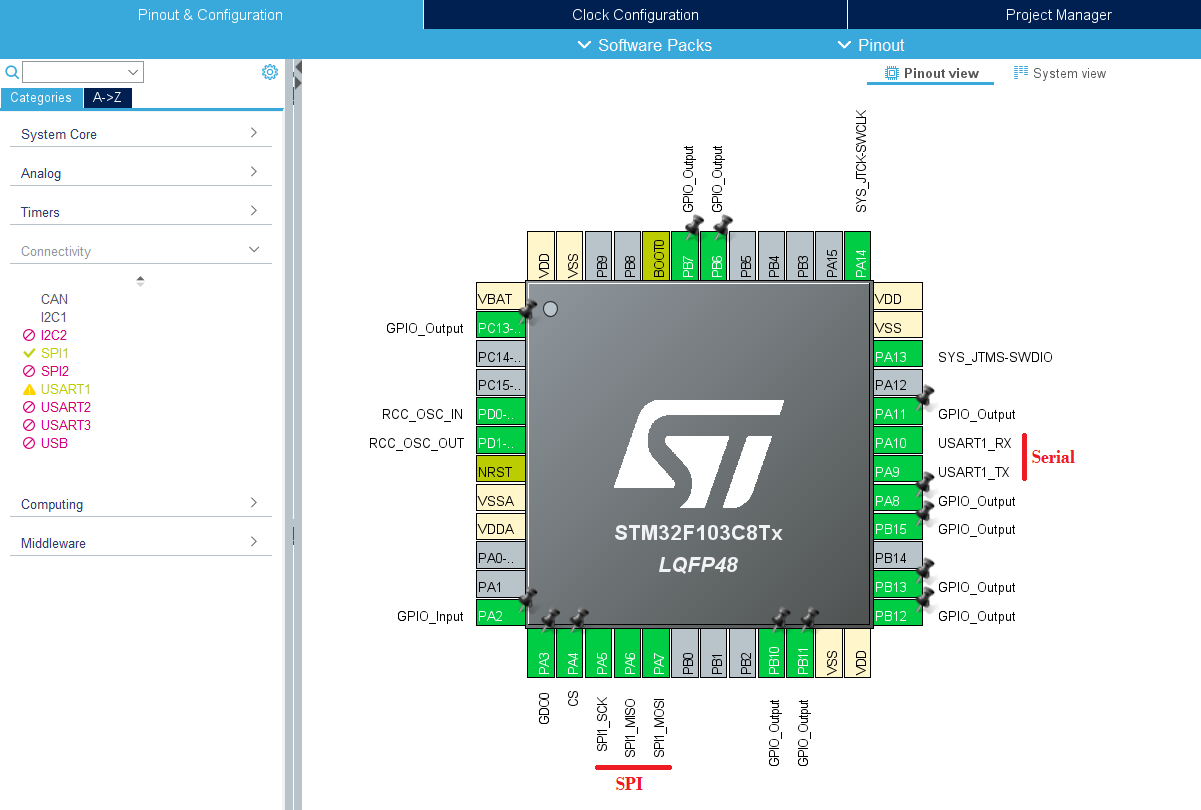
\includegraphics[scale=0.43]{images/nodos/asignacion_pines.png}
    \caption{Asignación de pines para comunicación}
	\label{asignacion_pines}
\end{figure}

Trabajar con este entorno es muy beneficioso ya que facilita en algunos aspectos la configuración del microcontrolador 
seleccionado, teniendo la capacidad de, mediante una interfaz gráfica, activar comunicaciones, configurar los relojes,
activar o desactivar interrupciones de timers y comunicaciones, entre otras. \par 
Las interrupciones en nuestro diseño juegan un papel clave debido a que en la comunicación se ha optado en algunos casos
particulares realizar el envío de los datos mediante interrupciones para que el procesador pueda continuar operando y no aboque 
todos sus recursos y tiempo de ejecución en enviar una palabra. De modo similar las interrupciones de timers nos han servido
para realizar acciones con alta prioridad y que deben ejecutarse en un tiempo específico, como por ejemplo la lectura asíncrona
de datos RAW enviados por un pin del CC1101. La configuración para las mismas se realiza de manera muy sencilla teniendo en 
cuenta la el contador de ticks del sistema, la frecuencia del clock utilizada y un preescaler a determinar para lograr el tiempo
deseado. \par 

\section{Diseño final}

El diseño el nodo ha surgido ciertas variaciones en el transcurso de la búsqueda del producto final. Entre estas se encuentra
la optimización del PCB reduciendo el tamaño del mismo, retirar los indicaores led, dotar la placa con el integrado destinado 
a la comunicación (SN75176). Para hacer un anális particular del funcionamiento del nodo hemos decidido analizar independientemente
el software del hardware.

\subsection{Software}

El nodo al ser el encargado de recibir la señal de RF, demodularla y determinar si hay o no inhibición posee una alta carga 
de software desarrollado sobre él. De este modo señalaremos particularmente el desarrollo en cada uno de los siguientes 
aspectos.

\begin{itemize}
	\item Recepción de RF.
	\item Estrategia de detección de inhibiciones.
	\item Comunicación con la central.
\end{itemize}

\subsubsection{Recepción RF}

El desarrollo de software en este aspecto cumple la necesidad que presenta el integrado receptor que utilizamos de ser 
configurado cada vez que este comienza a operar. Como previamente es analizado debemos establecer al dispositivo, que por
características es un transceptor, en modo de recepción. Además se debe configurar la frecuencia de operación, el modo de 
demodulación, el tipo de salida de datos, entre otras muchas cosas que son cargadas en un total de 46 registros. \par 
La carga de registros y el requerimiento de valor de RSSI que se le producen al CC1101 para tener noción de la potencia 
de RF en dBm que está llegando al receptor se realizan mediante comunicación SPI. Estos requerimientos son periódicos y 
han sido establecidos con un tiempo prudencial para que la comunicación resulte efectiva y los datos permanezcan actualizados.

\subsubsection{Estrategia de detección de inhibiciones}

La estrategia de detección de inhibiciones ha sido uno de los mayores desafíos a la hora de encarar el proyecto a causa de que
el sistema debe ser confiable y robusto para poder instalarlo en una zona de operación y que no tenga fallos. Principalmente
los errores de funcionamiento que son inadmisibles son: 
\begin{itemize}
	\item Falsas detecciones: que el sistema desate las alarmas cuando no hay presente un inhibidor o cuando en el canal se está
	comunicando un dispositivo que sí es apto para hacerlo, como por ejemplo una llave de auto.
	\item Falsos negativos: que el sistema sea incapaz de reconocer una señal que sea perjudicial para el sistema de seguridad
	dded un automóvil.
\end{itemize} 

Antes se ha profundizado en las estrategias de inhibición y se ha llegado a la conclusión de que existen dos métodos posibles
para inhibir una comunicación, un método es saturación de la etapa receptora y el otro es por corrupción de la trama de datos.
Para ambos métodos se ha debido realizar una estrategia de detección diferente, las cuales funcionan en simultáneo en el nodo
para desatar las alertas correspondientes si detectaran positivo. A continuación en las figuras \ref{estrategia_rssi} 
y \ref{estrategia_datos} se demuestra en bloques el funcionamiento de la estrategia de detección.

\begin{figure}
	\centering
	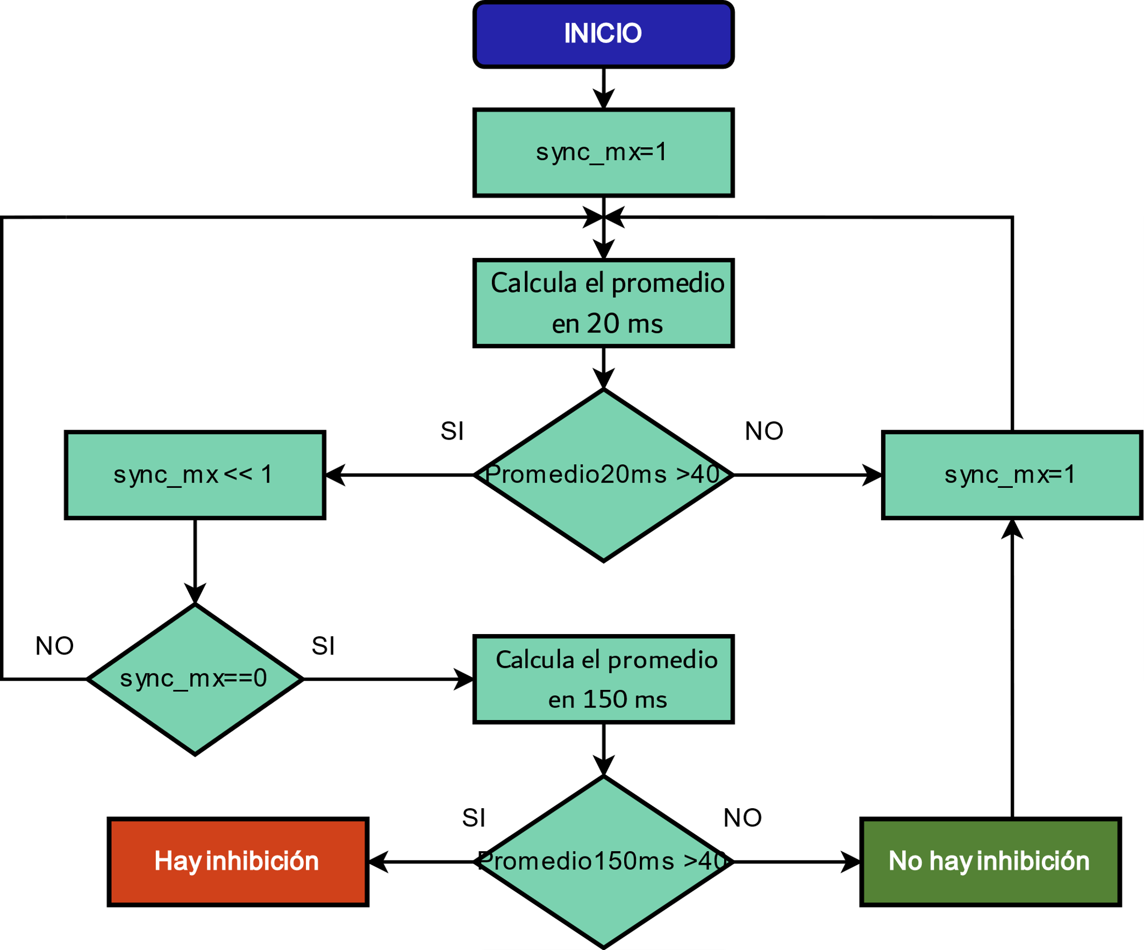
\includegraphics[scale=0.43]{images/nodos/estrategia_datos.png}
    \caption{Estrategia de detección por corrupción de datos}
	\label{estrategia_datos}
\end{figure}

\begin{figure}
	\centering
	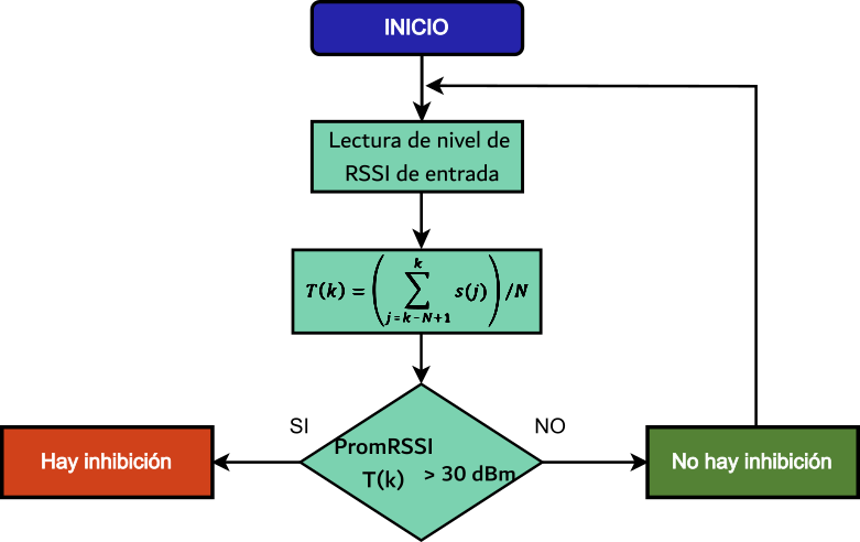
\includegraphics[scale=0.43]{images/nodos/estrategia_rssi.png}
    \caption{Estrategia de detección por saturación de etapa receptora}
	\label{estrategia_rssi}
\end{figure}

\subsubsection{Comunicación con la central}

Para el corriente funcionamiento del sistema se precisa que este se mantenga comunicado, dando información los nodos a la 
central de lo que cada uno están recibiendo, esta encargándose de manejar las alertas y los requerimientos a cada uno de los 
receptores. \par 
Para que la comunicación sea lo más efectiva posible se decidió que respete siempre una estructura de comunicación constante
en la que únicamente se cambirán los parámetros a enviar. La comunicación es del tipo master -la central- esclavos -los nodos-
y cada uno de los esclavos responderán por turno con peticiones independientes. \par
Como antes se mencionó la trama de comunicación es única y puede observarses en la figura \ref{comunicacion_nodo}, donde 
ID Nodo hace referencia al identificador propio del nodo en la red, Valor RSSI al valor de intensidad de señal recibido por cada
nodo y Estado hace referencia al estado de inhibición detectado, siendo 0 para no inhibición, 1 para inhibicion por corrupción
de datos y 2 para inhibición por saturación.

\begin{figure}
	\centering
	
\includegraphics[scale=0.43]{images/nodos/comunicacion_nodo.png}
    \caption{Estados de comunicación en nodo}
	\label{comunicacion_nodo}
\end{figure}


\subsection{Hardware}

En el nodo de recepción se hace uso del mismo MCU que en la central, de modo que las características de hardware antes mencionadas
tienen completa validez aquí también. Comunicado por SPI y comunicación serial se encuentra el módulo CC1101, luego mediante
comunicación serial asíncrona también tenemos el SN75176  

